\section{Trigeminal Neuralgia}

Neuralgias by definition are pain without any detectable physical origin, and originate from the brain. Trigeminal neuralgia (TN), or Tic douloureux, is a type of facial neuropathic pain that involves the trigeminal nerve. TN symptoms involve paroxysmal, shock-like pain condition affecting one or more of the three facial sensory nerve branches. The pain episodes can be unpredictable, as the length of episode can range from 1 to 1462 days \cite{Katusic1990}. Patients often describe its symptom as the most painful experience a human can undergo. Its physical and emotional disturbances are often severely disabling. 

The disorder has been documented as early as the first century AD, the clinical recognition of the disorder was by Nicolaus Andre in 1756, and by John Fothergill in 1776 \cite{Katusic1990}. In the three hundred years that followed, the aetiology of TN is still not completely understood. The modern understanding of the vascular compression of the trigeminal nerve root was first proposed by Janetta \cite{Jannetta1967}, where he elucidated that TN is a “nerve entrapment disorder” and that it may be a “consequence of aging … by arterialsclerotic elongation of the cerebrovasculature”.

Modern pain literature continuous to update the exactly diagnostic definition of TN. 

An older classification scheme divides facial pain into 5 major subtypes \cite{Burchiel2003,Eller2005}: idiopathic (without apparent cause), trigeminal injury, symptomatic, postherpetic, and atypical facial pain. Idiopathic TN has 2 sub-types: 1) TN type 1, where the patient experiences greater episodic pain greater than 50\% of the time; 2) TN type 2, where constant pain occurs greater than 50\% of the time. Trigeminal injury can be unintentional: which can be due to facial trauma, surgery to the oral cavity; this type of pain would involve persistent and burning pain to the affected areas; and is termed trigeminal neuropathic pain. The injury can also be intentional: due to interventions such as rhizotomy or gangliolysis; these result in numbness and loss of sensation of the face; and is termed trigeminal deafferentation pain. Symptomatic TN, also termed MS-TN, is due to trigeminal nerve injury relating to multiple sclerosis related central white matter inflammation. Postherpetic TN is pain resulting from the infection of the herpes zoster virus, and can involving burning pain and deafferentation. Atypical facial pain is classified as somatoform pain disorder that can be of psychosomatic origin, although some literature can also include constant pain in the face into this classification. 

The current The International Classification of Headache Disorders ICHD-3 Beta \cite{Society2013} classifies TN into classic TN, and painful trigeminal neuropathy. 
Classic TN's diagnostic criteria requires pain characteristics of: at least 3 attacks of unilateral facial pain; occuring in one or more trigeminal branches, with no radiation beyond the trigeminal distribution; severe intensity; electric shock-like, shooting, stabbing or sharp in quality; and precipatated by innocuous stimulation to the affected side of the face; and no clinically evident neurological deficit. Classic TN is further divided into purely paroxymal: recurrent attacks of unilateral facial pain with no persistent facial pain between attacks; and concomitant persistent: persistent facial pain of moderate intensity in the affected area. 
Painful trigeminal neuropathy in contrast are facial pain in one or more distributions of the trigeminal nerve caused by another disorder and indictive of neural damage. It can be further divided into categories relating to acute Herpes zoster, post-herpetic trigeminal neuropathy, multiple-sclerosis, space-occupying lesion, and other disorders.

There is also an definition \cite{Zakrzewska2016} that attempts to address the lack of symptomatic TN classification in ICHD-3 by classifying TN into idiopathic TN: without apparent cause; classic TN: caused by vascular compression of the trigeminal nerve root; and secondary TN: as the consequence of a major neurological disease such as MS. 

\subsection{Anatomy}

The trigeminal nerve, or the fifth cranial nerve (CN V) is the primary afferent for both facial somatosensation and pain (\ref{fig:trig-branches}). It consists of, from superior to inferior, the ophthalmic (V1), maxillary (V2) and mandibular (V3) branches. The distribution of the branches consists of both motor and sensory components. The motor branch of CN V activates the muscles responsible for mastication, as well as tensor tympani, tensor velipalatini, mylohyoid and anterior belly of the digastric. 

 \begin{figure}[ht]
 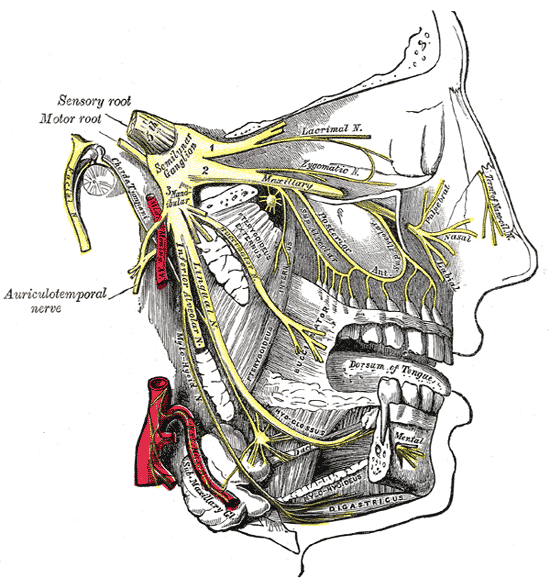
\includegraphics[width=120mm]{trig-branches.png}
 \centering
 \caption{Anatomy of the trigeminal nerve branches.} 
 \label{fig:trig-branches} 
 \end{figure}
 
The sensory afferents include the myelinated A and unmyelinated C-fibers that originate from the subcutaneous sensory receptors responsible for mechano and temperature pain, fine touch and vibration, such as the Messner's corpuscles, Pacinian and Ruffini corpuscles. 

The V1 branch provides the sensory innervation to the superior aspects of the face and cranium, including forehead, upper eyelids, eyeball, frontal sinus, lacrimal gland, and dura of the anteior cranial fossa. It further divides into lacrimal, frontal, and nasociliary nerve branches. The lacrimal branch supplies the lacrimal; the frontal contains smaller branches that innervates the skin of the medial forehead, upper eyelid, and parts of the frontal sinus; the nasociliary branch innervate various parts of the eye, and mucous membrane of the anterior nasal septum, anterior portion of the lateral nasal wall, and the skin on the tip of the nose. V1 enters the skull base through the superior orbital fissure.  

the V2 provides innervation to the temple, cheek, sides of the nose, and lower eyelids via the zygomaticofacial and zygomaticotemporal branches. It also innervates upper oral cavity. It enters through the foramen rotundum. 

V3 contains sensory and motor branches. It innervates skins of the jaw, areas above the ear, lips, gum, and teeth. The V3 division carries the mastication efferent to the four muscles recruited for mastications: the masseter, temporal, medial and lateral pterygoids. The tensor tympani also receives some CN V innervation, which is thought to be important in dampening the sound of chewing. V3 enters through foramen ovale. 

The branches then converge and form the trigeminal root gangion (TRG) (also known as Gasserian, or semilunar ganglion), whose posterior extension forms the CN V. It is analogous to the spinal dorsal root ganglion, and contains all the trigeminal sensory cell bodies. It situates in the meckel's cave, on the petrous bone of the middle cranial fossa. It is somatotomically organized in respect to the trigeminal branches, with V1 situated in medial anterior, V2 in caudal lateral, and V3 in the middle.

The extension of the posterior aspect of the TRG forms the trigeminal nerve body, with both sensory and motor roots. The nerve body straddles the TRG and the trigeminal nucleus, by crossing the pontine cistern. The portion of the sensory nerve that enters the pons is termed the trigeminal root entry zone (REZ). The cistern trigeminal sensory nerve, similar to other peripheral nerves, is myelinated by Schwann cells. The myelin cell type transitions to oligodendrocyte myelinations in the CNS as it enters the pons. The CNS myelin can be several millimetres beyond the surface of the pons, before it give away to the transition area, termed Obersteiner-Redlich zone \cite{Peker2006}.

 \begin{figure}[ht]
 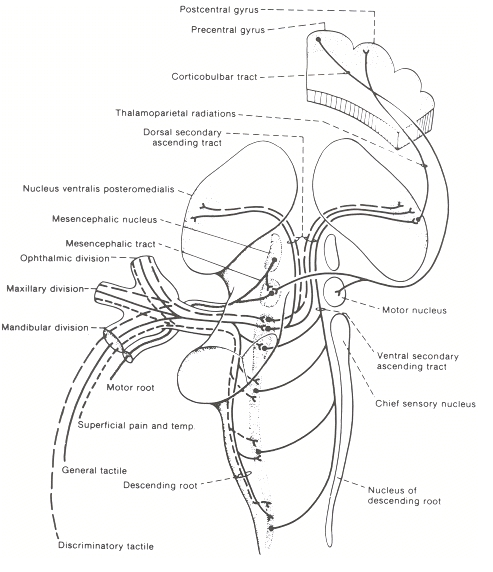
\includegraphics[width=100mm]{trig-pathway.png}
 \centering
 \caption{Overview of the trigeminal afferent pathways}
 \label{fig:trig-pathway}
 \end{figure}
 
The CN V passes into the pons (\ref{fig:trig-pathway}), through the pontine cerebellar peduncular bundles and enters the tegmentum of the pontine brainstem. CN V then curve towards the medial line before synapses onto the trigeminal nucleus in the basis of the pontine brainstem. The trigeminal nucleus is divided, from superior to inferior, into the mesencephalic, main sensory, and spinal nuclei. The spinal nucleus can be further divided into pars oralis, pars interpolaris and pars caudalis. 

The mesencephalic nucleus is responsible for proprioception, while the spinal trigeminal nucleus receives ipsilateral pain and temperature afferents not only from CN V, but also from CN VII, CN IX and CN X. Pars oralis transmits fine tactile sensations from the oralfacial region, pars interpolaris is also associated with dental pain, while pars caudalis is responsible for nociception and heat from the head. 

The main sensory nucleus receives discriminative somatosensation from the oralfacial region, and along with the spinal trigeminal nucleus fibers, project to the contralateral ventral caudal nucleus (VC) of thalamus by decussating at various levels of the pons via the anterior trigeminothalamic tract. A separate branch responsible for oral cavity however project to the ipsilateral VC via the dorsal trigeminothalamic tract.  

The VC thalamus projects to the primary sensory (S1) and secondary sensory (S2) cortical regions of the neocortex, thereby completing the afferent sensory projections of CN V. 



\subsection{Pathophysiology}

Classic TN is believed to be caused by neurovascular compression (NVC) of the CN V at its root entry zone (REZ) by the surrounding vasculature, where the nerve interfaces with the pons. An aberrant loop of artery and less commonly a vein is seen in 80-90\% of the cases of TN to compressing against the nerve \cite{Love2001,McLaughlin1999}. This can be observed in conventional MR imaging \cite{Borges2010}. Generally, the superior cerebellar artery is responsible for most of the NVC cases (60-90\%), and then the anteroinferior cerebellar artery and basilar arteries (Lutz et al., 2011). There is also evidence that TN is preferentially lateralized to the right side in 61\% of the cases, and in very rare cases may be related to asymmetries of the foramen rotundum and foramen ovale \cite{Toda2009}.  Other types of compressions may also cause TN, these can be in the forms of saccular aneurysm, arteriovenous malformation, vestibular schwannomas, meningiomas, epidermoid cysts, and other tumors.  However direct pathophysiological causal of TN pain is confounded by the fact observation of vascular compression does not always result in the expression of pain \cite{Desouza2013,Hodaie2013}. In some cases the TN pain is reported to be contralateral to the lesion \cite{Cheng2008,Haddad1990,Revuelta1995}. There are also 3.1-17\% of cases where TN occurs with no observable vascular compression \cite{Revuelta-Gutierrez2006}. 

Outside the brainstem, CN V is peripherally myelinated by Schwann cells, which are capable of remyelination. Inside the brainstem, the nerve is myelinated by oligodendrocytes. Study in 100 CN V samples from 50 cadavers \cite{Peker2006} showed that cisternal CN V length ranges from 8-15 mm; the transition zone length is shorter on the medial aspect (0.1-2.5 mm) than the lateral aspect (0.17-6.75 mm). The transition zone can be up to 25\% of the nerve length. 

The NVC that occurs in TN is believed to disrupt the central myelin, and that the region of disruption would begin at the peripheral-central myelin transition zone, and extending into central myelin regions. Janetta \cite{Jannetta1967} proposed that NVC leads to focal demyelination of the trigeminal sensory root axons, and causes ephaptic nerve conductances that cause neuralgia. Ultrastructural examinations \cite{Love1998} of tissue samples obtained from CN V rhizotomy specimens showed oligodendrocyte demyelination at the site of root transition zone. In TN, adjacent to the site of compression-related focal demyelination, were cases of thinly myelinated sheaths that encapsulates a number of demyelinated axons, suggesting aberrant remyelination. The TRG is also postulated to be responsible for neuralgia \cite{Rappaport1994}. It's believed that ganglionic ectopic autonomic firing can be trigged by mechanical disturbances as a result of nerve compression. Additionally, ganglionic cross aftercharge may occur as a result of repeated stimulations in the nerve injury site, which ignites surrounding ganglionic neurons. Histology findings by Devor et al supported the ignition hypothesis \cite{Devor2002a}, where demyelinated axons were shown to be in close apposition without intervening glia. 

\subsection{Treatment and outcomes}

For TN, anticonvulsant medication such as carbamazepine has 80\% response rate. However 50\% of patients will eventually need to undergo surgery as medication becomes ineffective due to tolerances. Nerve blocks such as peripheral neurectomy, neurolysis of the nerve or TRG can provide relief, albeit temporary, as pain always reoccurs \cite{Rappaport1994}. Long term treatment of TN involves the decompression of affected CN V \cite{Lovely1997}. This is achieved by either direct surgical intervention, in the form of microvascular decompression (MVD), where a Teflon\textcopyright padding is placed between the CN V root and the offending vessel. MVD showed 90\% pain relief immediately after surgery \cite{Zakrzewska2005}, and a long term success rate of 70\% at 10 years \cite{Barker1996}.
Partial sensory rhizotomy (PSR) can also be performed, where the offending CN V branch is severed, with a response rate of 88-70\% \cite{Young1993,Zakrzewska2005}. 

Intervation can also be non-invasive, in the form of GammaKnife radiosurgery (GKRS) \cite{Hodaie2012g}. The GK system focuses gamma radiation from approximately 200 cobalt-60 ($^{60}$Co) sources onto specific targets along the trigeminal nerve. Earlier targets focused on the trigeminal ganglion on adjacent areas \cite{Leksell1983}, while more proximal targets towards the brainstem is now recently used\cite{Daugherty2015}. Proximal targets correlate with longer pain relief, but also higher chance of facial numbness\cite{Xu2014}. The procedure requires a stereotactic frame, and a dose of 70-90 Gy is deposited. The effect is delayed and pain relief can be experienced in 4-6 weeks post-radiosurgery. GKRS treatments result in 90\% initial pain relief \cite{Regis2015,Kondziolka2010}, about 50-80\% pain free at 1 year, 45-65\% 2 years and 30-40\% 3 years after surgery \cite{Kondziolka2010,Sheehan2005}. More recent studies suggested higher pain free probabilities at 3(71.8\%), 5(64.9\%), 7(59.7\%) and 10(45.3\%) years\cite{Regis2015}. More favorable treatment outcomes were related to no other accompanying symptoms, no prior surgery and shorter term pain history of less than three years. 
